\PassOptionsToPackage{unicode=true}{hyperref} % options for packages loaded elsewhere
\PassOptionsToPackage{hyphens}{url}
%
\documentclass[ignorenonframetext,aspectratio=169,12pt]{beamer}
\usepackage{pgfpages}
\setbeamertemplate{caption}[numbered]
\setbeamertemplate{caption label separator}{: }
\setbeamercolor{caption name}{fg=normal text.fg}
\beamertemplatenavigationsymbolsempty
\usepackage{lmodern}
\usepackage{amssymb,amsmath}
\usepackage{ifxetex,ifluatex}
\usepackage{fixltx2e} % provides \textsubscript
\ifnum 0\ifxetex 1\fi\ifluatex 1\fi=0 % if pdftex
  \usepackage[T1]{fontenc}
  \usepackage[utf8]{inputenc}
  \usepackage{textcomp} % provides euro and other symbols
\else % if luatex or xelatex
  \usepackage{unicode-math}
  \defaultfontfeatures{Ligatures=TeX,Scale=MatchLowercase}
\fi
% use upquote if available, for straight quotes in verbatim environments
\IfFileExists{upquote.sty}{\usepackage{upquote}}{}
% use microtype if available
\IfFileExists{microtype.sty}{%
\usepackage[]{microtype}
\UseMicrotypeSet[protrusion]{basicmath} % disable protrusion for tt fonts
}{}
\IfFileExists{parskip.sty}{%
\usepackage{parskip}
}{% else
\setlength{\parindent}{0pt}
\setlength{\parskip}{6pt plus 2pt minus 1pt}
}
\usepackage{hyperref}
\hypersetup{
            pdfborder={0 0 0},
            breaklinks=true}
\urlstyle{same}  % don't use monospace font for urls
\newif\ifbibliography
% Prevent slide breaks in the middle of a paragraph:
\widowpenalties 1 10000
\raggedbottom
\setbeamertemplate{part page}{
\centering
\begin{beamercolorbox}[sep=16pt,center]{part title}
  \usebeamerfont{part title}\insertpart\par
\end{beamercolorbox}
}
\setbeamertemplate{section page}{
\centering
\begin{beamercolorbox}[sep=12pt,center]{part title}
  \usebeamerfont{section title}\insertsection\par
\end{beamercolorbox}
}
\setbeamertemplate{subsection page}{
\centering
\begin{beamercolorbox}[sep=8pt,center]{part title}
  \usebeamerfont{subsection title}\insertsubsection\par
\end{beamercolorbox}
}
\AtBeginPart{
  \frame{\partpage}
}
\AtBeginSection{
  \ifbibliography
  \else
    \frame{\sectionpage}
  \fi
}
\AtBeginSubsection{
  \frame{\subsectionpage}
}
\setlength{\emergencystretch}{3em}  % prevent overfull lines
\providecommand{\tightlist}{%
  \setlength{\itemsep}{0pt}\setlength{\parskip}{0pt}}
\setcounter{secnumdepth}{0}

% set default figure placement to htbp
\makeatletter
\def\fps@figure{htbp}
\makeatother

\DeclareUnicodeCharacter{00A0}{~}
\DeclareUnicodeCharacter{03B4}{$\delta$}
\DeclareUnicodeCharacter{03B5}{$\varepsilon$}
\DeclareUnicodeCharacter{03C9}{$\omega$}
\DeclareUnicodeCharacter{2124}{\mathbb{Z}}
\DeclareUnicodeCharacter{2193}{$\downarrow$}
\DeclareUnicodeCharacter{2208}{$\in$}
\DeclareUnicodeCharacter{2209}{$\notin$}
\DeclareUnicodeCharacter{220B}{$\ni$}
\DeclareUnicodeCharacter{2227}{$\wedge$}
\DeclareUnicodeCharacter{2228}{$\vee$}
\DeclareUnicodeCharacter{2234}{$\therefore$}
\DeclareUnicodeCharacter{2264}{$\leq$}
\DeclareUnicodeCharacter{2265}{$\geq$}
\DeclareUnicodeCharacter{2605}{$\star$}
\DeclareUnicodeCharacter{1D53D}{\mathbb{F}}

% Scale images if necessary, so that they will not overflow the page
% margins by default, and it is still possible to overwrite the defaults
% using explicit options in \includegraphics[width, height, ...]{}
%\setkeys{Gin}{width=\maxwidth,height=\maxheight,keepaspectratio}
\newcommand{\includegraphicsscaled}[1]{
    \includegraphics[width=\maxwidth,height=\maxheight,keepaspectratio]{#1}
}


\hypersetup{colorlinks,linkcolor=,urlcolor=purple}
\setbeamertemplate{navigation symbols}{}
\usefonttheme[onlymath]{serif}

\setbeamercolor{footnote mark}{fg=gray}
\setbeamerfont{footnote}{size=\tiny}
\usepackage{color}
\usepackage[normalem]{ulem}
\usepackage{listings}
\lstset{
    basicstyle=\ttfamily\normalsize,
    keywordstyle=\color{blue}\bfseries,
    commentstyle=\color[rgb]{0,0.5,0}\bfseries\em,
    stringstyle=\color{red}\bfseries\em,
    escapeinside={(*}{*)}
}

\usepackage{graphicx,grffile}
\makeatletter
\def\maxwidth{\ifdim\Gin@nat@width>\linewidth\linewidth\else\Gin@nat@width\fi}
\def\maxheight{\ifdim\Gin@nat@height>\textheight\textheight\else\Gin@nat@height\fi}
\makeatother

\title{\bf Haskell Security Response Team---2 years on}
\providecommand{\subtitle}[1]{}
\subtitle{doings, learnings, dreamings}
\author{{\bf Fraser Tweedale}\\
    \texttt{@hackuador@functional.cafe}}
\date{2025-05-13}

\begin{document}
\frame{\titlepage}

\begin{frame}{Outline}
    \begin{itemize}
        \item Why security response matters
        \item Building and running a security team
        \item The advisory database
        \item Ongoing / future developments
        \item Sustainability
    \end{itemize}
\end{frame}


\begin{frame}[plain]
\begin{center}
    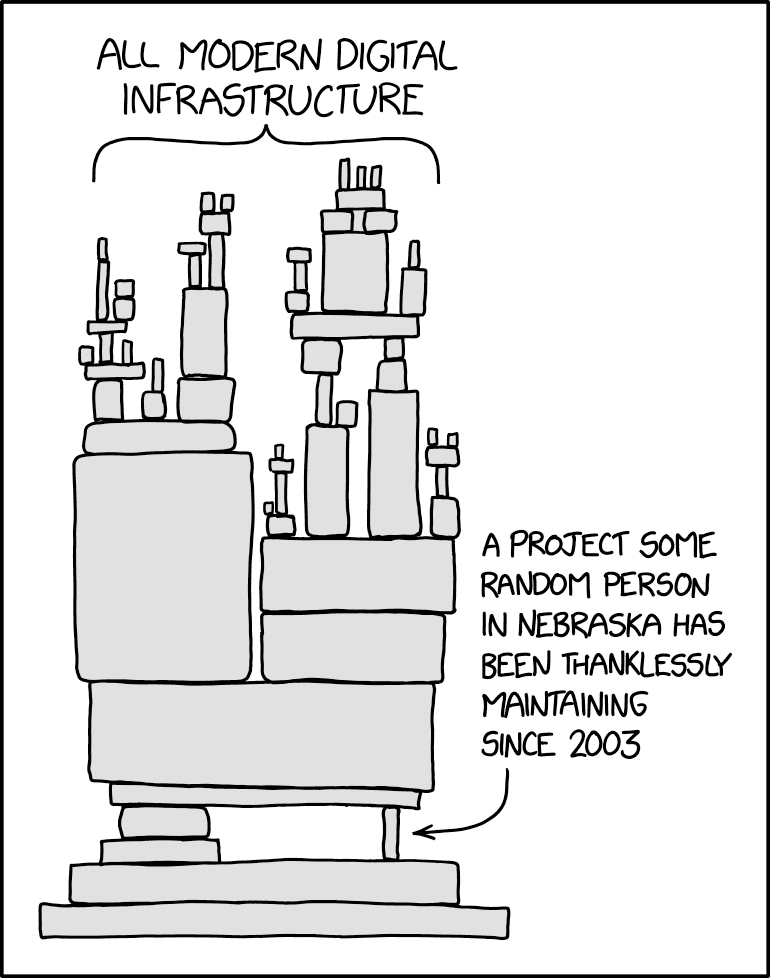
\includegraphics[height=0.9\maxheight,keepaspectratio]{dependency_2x.png}
    \\
    \tiny
    CC-BY-NC 2.5 \texttt{\url{https://xkcd.com/2347/}}
\end{center}
\end{frame}

\begin{frame}{Why open source security matters}
    \begin{itemize}
        \item supply chain security
        \item ISO 27001 de-risking
        \item NIST SP 800-218 (SSDF)
            \footnote{\url{https://csrc.nist.gov/pubs/sp/800/218/final}}
            + EO 14028 (procurement)
            \footnote{\url{https://www.nist.gov/system/files/documents/2022/02/04/software-supply-chain-security-guidance-under-EO-14028-section-4e.pdf}}
        \item EU Cyber Resilience Act
            \footnote{\url{https://eur-lex.europa.eu/legal-content/EN/TXT/HTML/?uri=OJ:L_202402847&qid=1732732976975\#art_24}}
            \footnote{\url{https://github.blog/open-source/maintainers/what-the-eus-new-software-legislation-means-for-developers/}}
    \end{itemize}
\end{frame}

\begin{frame}{Why open source security matters}
\begin{quote}
\raggedright
  Open-source software {stewards} shall put in place\ldots{}
  a {cybersecurity policy} to foster\ldots{}
  effective {handling of vulnerabilities}\ldots{}
  also foster the {voluntary reporting} of vulnerabilities\ldots{}
  promote the {sharing of information} concerning discovered vulnerabilities
\\
  {\hfill --- \footnotesize Cyber Resilience Act, Article 24 {\em
  \textbf{Obligations of open-source software stewards}}}
\end{quote}
\end{frame}

\begin{frame}{Why open source security matters}
\large
\begin{quote}
\raggedright
Supply chain security has always been important.  But market
  participants and open source organisations care more now (because
  they've been forced to).

\bigskip

Therefore, open source projects and ecosystems that lack an
effective security apparatus will be left behind.
\end{quote}
\end{frame}

\begin{frame}{Who needs a security response apparatus?}
    \begin{itemize}
        \item operating systems
        \item programming languages + library ecosystems
        \item frameworks
        \item applications + network servers
        \item other large projects
    \end{itemize}
\end{frame}

\begin{frame}{Haskell Security Response Team (SRT)}
  \begin{itemize}
    \item Haskell Foundation {\em tech proposal}
          \footnote{\url{https://github.com/haskellfoundation/tech-proposals/blob/main/proposals/accepted/037-advisory-db.md}}
    \item I was asked to recruit and lead the team
  \end{itemize}
\end{frame}

\begin{frame}{SRT - scope}
    \begin{itemize}
        \item Manage the advisory database and associated tooling
        \item Triage, assess and admit issue reports
        \item Coordinate repsonse with maintainers of affected
            packages (high-impact issues)
        \item Collaborate and respond to needs of downstream tools
            that consume our advisories
        \item Quarterly report
    \end{itemize}
\end{frame}


\section{Building and running a security team}

\begin{frame}{Building a team - skills}
    \begin{itemize}
        \item technical skills / knowledge of the language / project
        \item security know-how: AppSec, IR, GRC, pen
          testing, IAM, vuln research, \ldots{}
        \item programming ability (for tool development)
        \item good communication skills
    \end{itemize}
\end{frame}

\begin{frame}{Building a team - how many?}
    \begin{itemize}
        \item enough to cover the skills you want / need
        \item enough to tolerate absences
        \item {\bf not all} the qualified people all at once
        \item diversity is good!
        \item {\em Haskell: currently 6 people}
    \end{itemize}
\end{frame}

\begin{frame}{Defining the scope of work}
  \begin{itemize}
    \item triage security reports
      \begin{itemize}
        \item analyse reports and propose action
        \item coordinate with maintainers and stakeholders
      \end{itemize}
    \item publish advisories
    \item oversee project infrastructure security
    \item developer tooling
    \item reports, guides, documentation, \ldots{}
  \end{itemize}

  You can't do everything.  Choose a scope and review it regularly.
\end{frame}

\begin{frame}{Building a team - call for volunteers}
  \begin{itemize}
    \item preamble
    \item team responsibilities
    \item desired skills / experience
    \item how to apply
    \item {\em Haskell SRT example}\footnote{\url{https://github.com/haskell/security-advisories/blob/main/docs/call-for-volunteers-example.md}} (feel free to copy!)
  \end{itemize}
\end{frame}

\begin{frame}{Processes and communication}
    \begin{itemize}
        \item reporting and disclosure processes
        \item team chat / mailing list (private!)
        \item meetings ({\em Haskell: every 2 weeks})
        \item activity reports ({\em Haskell: quarterly})
        \item community engagement (conferences, discussions, office hours)
    \end{itemize}
\end{frame}

\begin{frame}{Embargoed advisories}
  \begin{itemize}
    \item what threshold for embargo? (you decide)
    \item notifying downstream {\bf redistributors} (e.g. Linux distros)
    \item multi-ecosystem vulnerabilities
    \item {\em Vulnerability Information and Coordination
      Environment (VINCE)}\footnote{\url{https://kb.cert.org/vince/}}
      \begin{itemize}
        \item enable secure reporting and cross-vendor collab
        \item register your project / ecosystem!
      \end{itemize}
  \end{itemize}
\end{frame}

\begin{frame}{Bug bounties and audits}
  \begin{itemize}
    \item if you can fund them, great
    \item fund security response capacity first!
    \item Haskell: maybe one day :(
  \end{itemize}
\end{frame}



\section{The advisory database}

\begin{frame}{Advisory database - structure}
  \begin{itemize}
    \item \url{https://github.com/haskell/security-advisories}
    \item TOML metadata + CommonMark description
    \item arranged by namespace and package/component name
    \item symlinks for multi-package advisories
    \item quirk: dates are derived from Git commit times
  \end{itemize}
\end{frame}

\begin{frame}{Advisory naming}
  \begin{itemize}
    \item some ecosystems/projects use own namespace
      (e.g. {\em HSEC-YYYY-NNNN})
    \item some are a CVE Numbering Authority (CNA)
        \footnote{\url{https://github.com/ossf/wg-vulnerability-disclosures/blob/main/docs/guides/becoming-a-cna-as-an-open-source-org-or-project.md}}
      \begin{itemize}
        \item {\bf suppress bogus CVEs}
          \footnote{\url{https://lwn.net/Articles/961978/}}
        \item produce higher-quality CVE records
      \end{itemize}
    \item some use existing CNAs
  \end{itemize}
\end{frame}

\begin{frame}{Advisory content}
  \begin{itemize}
    \item description (give detail!)
    \item affected packages and versions
    \item CVSS, CWE
    \item aliases and related IDs
    \item references (reports, PoC, commits, \ldots{})
  \end{itemize}
\end{frame}


\begin{frame}[fragile]
\scriptsize
\begin{verbatim}
```toml
[advisory]
id = "HSEC-2023-0001"
cwe = [328, 400]
keywords = ["json", "dos", "historical"]
aliases = ["CVE-2022-3433"]

[[affected]]
package = "aeson"
cvss = "CVSS:3.1/AV:N/AC:L/PR:L/UI:N/S:U/C:N/I:N/A:H"

[[affected.versions]]
introduced = "0.4.0.0"
fixed = "2.0.1.0"
```

# Hash flooding vulnerability in aeson

*aeson* was vulnerable to hash flooding (a.k.a. hash DoS).  The
issue is a consequence of the HashMap implementation from
*unordered-containers*.  It results in a denial of service through
CPU consumption.  This technique has been used in real-world attacks
against a variety of languages, libraries and frameworks over the
years.

\end{verbatim}
\end{frame}

\begin{frame}{Advisory database - outputs}
  \begin{itemize}
    \item OSV (ingested by
      osv.dev\footnote{\url{https://osv.dev/list?ecosystem=Hackage}})
    \item HTML index: \url{https://haskell.github.io/security-advisories/}
    \item "snapshot" format designed for syncing with
      tools\footnote{\url{https://github.com/haskell/security-advisories/pull/179}}
  \end{itemize}
\end{frame}

\begin{frame}{Advisory database - libraries}

  Libraries and tools for processing advisory data are on Hackage:

  \begin{itemize}
    \item \url{https://hackage.haskell.org/package/cvss}
    \item \url{https://hackage.haskell.org/package/osv}
    \item \url{https://hackage.haskell.org/package/hsec-core}
    \item \url{https://hackage.haskell.org/package/hsec-tools}
  \end{itemize}

  Expect churn as more consumers/users arrive, give feedback.

  CWE\footnote{{\em Common Weakness Enumeration}---\url{https://cwe.mitre.org/}} library is coming.

\end{frame}


\section{What the advisories tell us}

\begin{frame}{Advisory database - the numbers (May 2025)}
  \begin{itemize}
    \item 26 advisories published
    \item 23 affecting packages on Hackage, 3 for GHC toolchain
    \item some advisories affect multiple packages/components
    \item 2 HSEC IDs reserved (embargoed issues)
  \end{itemize}
\end{frame}

\begin{frame}{Most common vulnerability types}
  \begin{itemize}
    \item RCE / command injection
    \item deserialisation issues (hash flooding, entity expansion, etc)
    \item cross-site scripting (XSS)
    \item numeric conversion issues
    \item issues in stale bundled C libs
    \item logic errors and boolean blindness
  \end{itemize}

  Takeaway: we have big blind spots!  Strong type system is no
  panacea.
\end{frame}

\begin{frame}{Less common vulnerability types}
  \begin{itemize}
    \item type confusion
    \item memory corruption (modulo bundled cbits)
    \item null pointer dereference
    \item SQLi? (none reported, so far)
  \end{itemize}
\end{frame}

\section{Ongoing / future developments}

\begin{frame}{cabal-audit}
  \begin{itemize}
    \item Scans the build plan for vulnerable dependencies
    \item Long-term goal: integrated with {\tt cabal-install} (as
      plugin)
      \begin{itemize}
        \item Ship via GHCUp?
      \end{itemize}
    \item \url{https://github.com/MangoIV/cabal-audit}
  \end{itemize}
\end{frame}

\begin{frame}[plain]
  \begin{center}
    \includegraphicsscaled{cabal-audit-screenshot.png}
  \end{center}
\end{frame}

\begin{frame}{{\bf Hackage} - integrate with advisory db}
  \begin{itemize}
    \item Show info about vulnerable versions
    \item Show info about (potentially) vulnerable deps
    \item Add "how to report" info / helpers
    \item Flora.pm has some preliminary integration
  \end{itemize}
\end{frame}

\begin{frame}{{\bf Hackage} - other security enhancements}
  \begin{itemize}
    \item password / token storage improvements
    \item 2FA (TOTP for a start)
  \end{itemize}
\end{frame}

\begin{frame}{SRT tooling}
  \begin{itemize}
    \item CVSS 4.0 support
    \item {\bf GitHub bot} to help define / review advisories
      \begin{itemize}
        \item explain CVSS, CWE values; suggest keywords; etc
      \end{itemize}
    \item {\bf Web form} for advisory submission
      \begin{itemize}
        \item \ldots{}or other ways to make it easier
      \end{itemize}
  \end{itemize}
\end{frame}

\begin{frame}{Exploitability information}
  \begin{itemize}
    \item As audit tooling matures, we must suppress false positives
      \begin{itemize}
        \item e.g. HSEC-2023-0007 {\tt readFloat} memory exhaustion
          in {\em \textbf{base}}
      \end{itemize}
      
    \item VEX - {\em Vulnerability Exploitability eXchange}
      \begin{itemize}
        \item statements that an issue is(n't) exploitable in the
          dependent
        \item {\bf data model} by CISA.gov
        \item implementations:
          \href{https://github.com/openvex/spec}{OpenVEX},
          \href{https://spdx.dev/capturing-software-vulnerability-data-in-spdx-3-0/}{SPDX 3.0},
          \href{https://www.oasis-open.org/2022/11/21/new-version-of-csaf-standard/}{OASIS CSAF 2.0},
          CycloneDX 
      \end{itemize}
    \item We don't have to use VEX {\em per se}
  \end{itemize}
\end{frame}

\begin{frame}{VEX statements - generation}
  \begin{itemize}
    \item Written by human
    \item Generated by machine (call analysis)
      \begin{itemize}
        \item Tristan's experiment: \url{https://github.com/TristanCacqueray/cabal-audit}
        \item typeclass methods seem to be the tricky part
        \item relies on declaration of affected
          functions/symbols in the advisory
      \end{itemize}
  \end{itemize}
\end{frame}

\begin{frame}{VEX statements - distribution}
  \begin{itemize}
    \item Cabal package description ({\bf dependent})
      \begin{itemize}
        \item supplied by maintainer, or Hackage trustees
        \item distributed in Hackage snapshots
        \item metadata revisions $\to$ new version not required to
          update VEX statements
      \end{itemize}
    \item Advisory DB as a VEX clearing-house
      \begin{itemize}
        \item supplied by SRT, or community with SRT review
        \item distributed in Advisory DB snapshots
      \end{itemize}
    \item Both?
      \begin{itemize}
        \item requires conflict resolution (preferred source)
      \end{itemize}
  \end{itemize}
\end{frame}

\begin{frame}{Dependency graph analysis}
  \begin{itemize}
    \item Tools to analyse the dependency graph (of a single project
      or whole ecosystem) are increasingly important
    \item That xkcd\footnote{\url{https://xkcd.com/2347/}}
    \item Identify the {\bf load-bearing projects / juicy targets}?
      \begin{itemize}
        \item Are they maintained?  Sustainably?
        \item What are the main risks?
      \end{itemize}
    \item Query projects exposed to {\bf external risks}
      \begin{itemize}
        \item cbits?  vendored/bundled code?  out of date?
        \item using external libraries?
      \end{itemize}
  \end{itemize}
\end{frame}

\begin{frame}{Dependency graph analysis - Open Source Insights}
  \begin{itemize}
    \item A fair bit of this tooling exists in
      {\em Open Source Insights}
      \begin{itemize}
        \item \url{https://deps.dev}; Google project
        \item Web, visualisations, API, BigQuery
      \end{itemize}
    \item Haskell is not supported yet
    \item Development is not public (currently)
    \item \href{https://hackage.haskell.org/package/acme-everything}
      {\em acme-everything} becomes useful?
  \end{itemize}
\end{frame}

\begin{frame}{But wait there's more\ldots{}}
  \begin{itemize}
    \item SBOM artifacts? (e.g. \href{https://spdx.dev/}{SPDX})
    \item Add Haskell call analysis support to
      \href{https://google.github.io/osv-scanner}{osv-scanner}?
    \item Increase issue discovery efforts
      \begin{itemize}
        \item \href{https://github.com/google/oss-fuzz}{OSS-Fuzz} support?
      \end{itemize}
    \item \href{https://www.bestpractices.dev/en/criteria/0}{OpenSSF Best Practices} checking?
  \end{itemize}
\end{frame}

\begin{frame}{Software Bill of Materials (SBOM)}
  \begin{itemize}
    \item Blog post published yesterday:
      \begin{itemize}
        \item {\em SBOM Generation and Vulnerability Monitoring for
          the Hackage/Haskell Ecosystem}\footnote{\url{https://www.timesys.com/security/sbom-generation-and-vulnerability-monitoring-for-the-hackage-haskell-ecosystem/}}---Timesys (cybersecurity
          vendor)
        \item Cabal freeze file $\to$ CycloneDX SBOM via
          {\em syft}\footnote{\url{https://github.com/anchore/syft}}
      \end{itemize}
    \item Build SBOM generation into {\tt cabal-install}?  As
      plugin?
  \end{itemize}
\end{frame}


\section{Sustainability}

\begin{frame}{A not good scenario}
  \begin{itemize}
    \item critical issue disclosed
    \item requires significant effort and coordination
    \item everyone is busy with their day job and life
    \item issue remains unfixed\ldots{}
  \end{itemize}

  This is where Haskell is at :(
\end{frame}

\begin{frame}{Bottom line}
\large
\begin{quote}
\raggedright
  Open source ecosystems need personnel with {\bf capacity} and
  {\bf authority} to respond {\bf immediately} to security incidents.
\end{quote}
\end{frame}

\begin{frame}{How commercial users can help}
  \begin{itemize}
    \item Support the Haskell Foundation!
    \item Give developer time to high-impact security work
    \item Fund security audits of critical tools/libs
  \end{itemize}
\end{frame}

\begin{frame}{Subscription model?}
  \begin{itemize}
        \item commercial users directly fund security work; in
          return you get…
          \begin{itemize}
            \item a heads-up on active issues
            \item a say in priorities, tooling
            \item access to team for advice/consulting
          \end{itemize}
  \end{itemize}

  Might be a possibility?  Are you interested?
\end{frame}




% END MATTER

\begin{frame}[plain]
\begin{columns}

  \begin{column}{.6\textwidth}

    \setlength{\parskip}{.5em}

    { \centering

    \input{cc-by-ARTIFACT.pdf_tex}

    \copyright~2025  Fraser Tweedale

    { \scriptsize
    Except where otherwise noted this work is licensed under
    }
    { \footnotesize
    \textbf{http://creativecommons.org/licenses/by/4.0/}
    }

    }

    \begin{description}
      \small
      \item[SRT web] \url{https://www.haskell.org/security/}
      \item[My blog] \href{https://frasertweedale.github.io/blog-fp/}{frasertweedale.github.io/blog-fp}
      \item[Fediverse] \href{https://functional.cafe/@hackuador}{@hackuador@functional.cafe}
    \end{description}
  \end{column}

\end{columns}
\end{frame}

\end{document}
